\usepackage{tikz}

%<*USAR Initial Action>
\section{USAR Initial Action}
	\begin{itemize}
		\item Strategies
		\item Size up scene
		\item Implement CIMS
		\item Set up communications quickly
		\item Send SITREP to base/dispatch
		\item Request specialist assistance
		\item R-E-P-E-A-T
		\item Constantly gather information
		\item Limit supervisory staff in logistics
		\item Centralise logistics
		\item Use an inventory control system
		\item Determine the length of the incident
		\item Plan ahead – logistics, personnel \& welfare
	\end{itemize}
%</USAR Initial Action>

%<*REPEAT>
\section{R-E-P-E-A-T}
	\begin{description}
		\item[R]econnaissance
		\item[E]limination of services
		\item[P]rimary surface search
		\item[E]xploration of voids
		\item[A]ccess by selected debris removal
		\item[T]erminate by general debris removal
	\end{description}
%</REPEAT>

%<Floor Identification>
\section{Floor Identification}
	\begin{tabular}{|c|}
		\hline
		Floor 2 \\
		\hline
		Floor 1 \\
		\hline
		Ground Floor \\
		\hline
		Basement 1 \\
		\hline
		Basement 2
	\end{tabular}

%<ID>
%<Geographical ID>
\section{Geographical ID}
	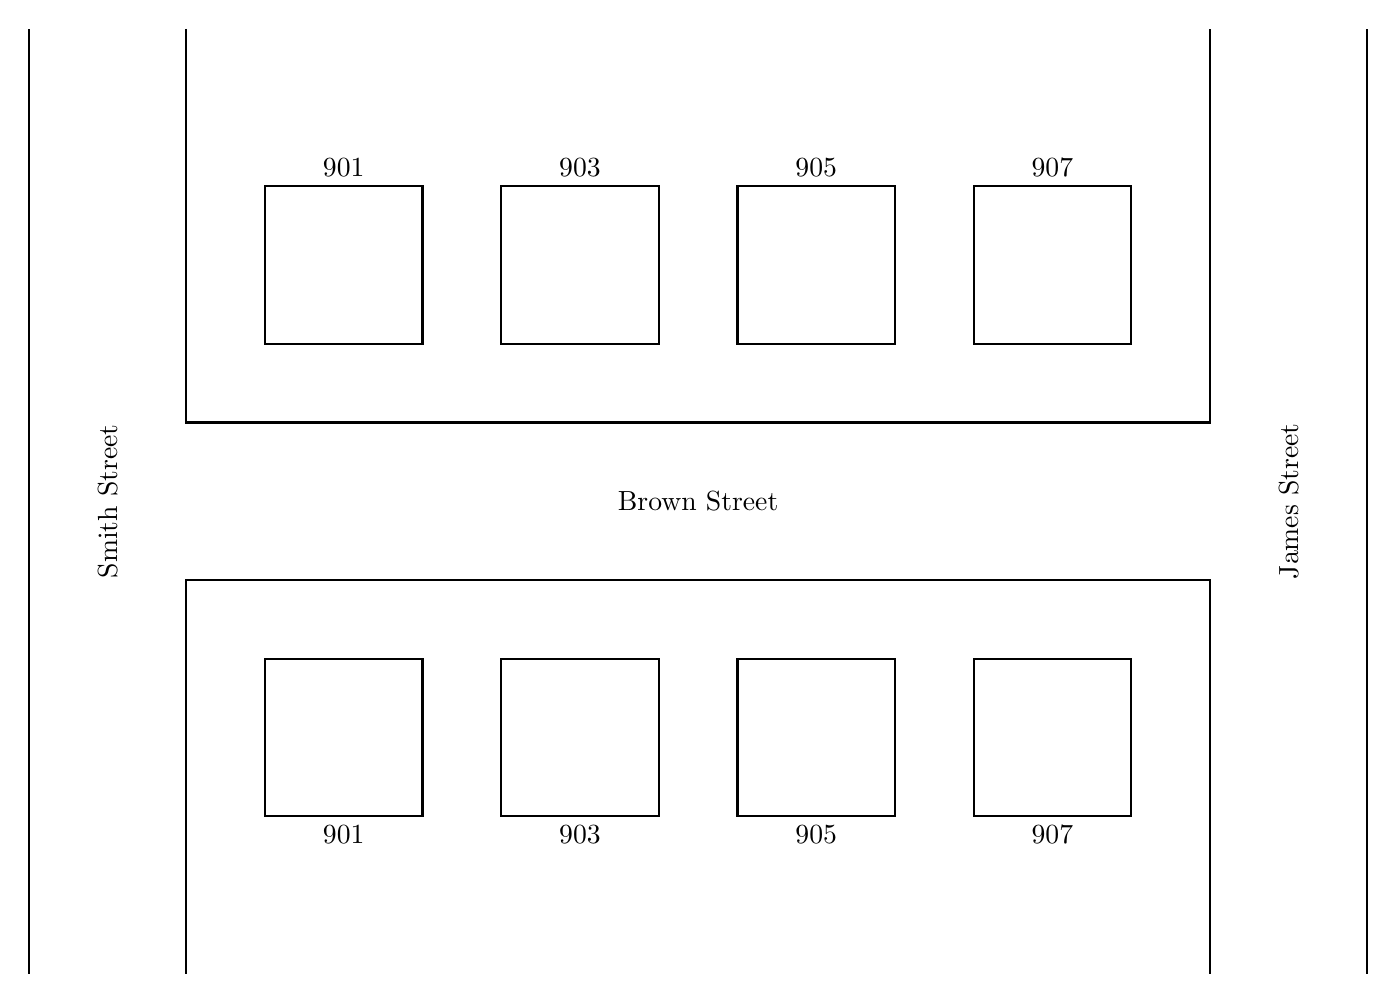
\begin{tikzpicture}
		\draw [thick] (0,0) -- (0,12);
		\draw [thick] (17,0) -- (17,12);
		\draw [thick] (2,0) -- (2,5) -- (15,5) -- (15,0);
		\draw [thick] (2,12) -- (2,7) -- (15,7) -- (15,12);
		\node at (8.5,6) {Brown Street};
		\node [rotate=90] at (1,6) {Smith Street};
		\node [rotate=90] at (16,6) {James Street};
		\draw [thick] (3,2) rectangle (5,4);
		\node [below] at (4,2) {901};
		\draw [thick] (6,2) rectangle (8,4);
		\node [below] at (7,2) {903};
		\draw [thick] (9,2) rectangle (11,4);
		\node [below] at (10,2) {905};
		\draw [thick] (12,2) rectangle (14,4);
		\node [below] at (13,2) {907};
		\draw [thick] (3,8) rectangle (5,10);
		\node [above] at (4,10) {901};
		\draw [thick] (6,8) rectangle (8,10);
		\node [above] at (7,10) {903};
		\draw [thick] (9,8) rectangle (11,10);
		\node [above] at (10,10) {905};
		\draw [thick] (12,8) rectangle (14,10);
		\node [above] at (13,10) {907};
	\end{tikzpicture}
	\textbf{NOTE:} Primary geographical ID shall be the existing street name and
	building number. Attempt to re-establish existing numbering system. Front of
	structures to be clearly marked using international orange spray paint. The
	boundary frontage of individual structures should be indicated using barrier
	tape or spray paint.
%</Geographical ID>

%<Sectoring ID - Sides>
\section{Sectoring ID - Sides}
	\begin{tikzpicture}
		\draw (0,0) -- (17,0);
		\node at (8.5,1) {700 Block Alpha Street};
		\draw (2,0) -- (17.2);
		\draw [thick] (4,4) rectangle (13,8);
		\node [below] at (8.5,4) {Side One};
		\node [left] at (4,6) {Side\\Two};
		\node [above] at (8.5,8) {Side Three};
		\node [right] at (13,6) {Side\\Four};
	\end{tikzpicture}
%<Sectoring ID - Sides>

%<Sectoring ID - Quadrants>
\section{Sectoring ID - Quadrants}
	\begin{tikzpicture}
		\draw (0,0) -- (17,0);
		\node at (8.5,1) {700 Block Alpha Street};
		\draw (2,0) -- (17.2);
		\draw [thick] (4,4) rectangle (13,8);
		\draw [thick] (7,5) rectangle (10,7);
		\node at (8.5,6) {E};
		\draw [thick] (4,6) -- (7,6);
		\draw [thick] (10,6) -- (13,6);
		\draw [thick] (8.5,4) -- (8.5,5);
		\draw [thick] (8.5,7) -- (8.5,8);
	\end{tikzpicture}
		
%</Sectoring ID - Quadrants>


%</ID>
